\input{../slides/common/slides_common}

\newif\ifbook
\input{../shared/chisel}

% TikZ for diagrams
\usepackage{tikz}
\usetikzlibrary{positioning, arrows.meta}

% Optional visual tweaks
\tikzset{
    >=Stealth,
    every node/.style={rounded corners=2pt}
}

\title{Generators}
\author{Martin Schoeberl}
\date{\today}
\institute{Technical University of Denmark\\
Embedded Systems Engineering}

\begin{document}

\begin{frame}
\titlepage
\end{frame}

\begin{frame}[fragile]{Overview}
\begin{itemize}
\item Functions with more outputs
\item Solution to the min/max lab
\item Type conversions
\item Parameters (simple and types)
\item More Scala for generators
\end{itemize}
\end{frame}

\begin{frame}[fragile]{Functions with Multiple Outputs}
\begin{itemize}
\item We use functions to generate hardware
\item The return value is the \emph{output} of that \emph{module}
\item A function usually has a single return value
\item Use a Scala tuple for more output \emph{ports}
\shortlist{../code/fun_comp.txt}
\end{itemize}
\end{frame}

\begin{frame}[fragile]{Functions with More Outputs}
\begin{itemize}
\item Access the two output wires with the \code{.\_n} syntax.
\shortlist{../code/fun_comp_use1.txt}
\item Or directly decompose the tuple
\shortlist{../code/fun_comp_use2.txt}
\item Functions can be declared as part of a \code{Module}
\item Better place them into a Scala object collecting utility functions
\item Functions can serve as ligthweight modules
\end{itemize}
\end{frame}

\begin{frame}[fragile]{Lab two Weeks Ago}
\begin{itemize}
\item Write a search for the minimum circuit (with \code{treeReduce()})
\item Add the generation of the index of the minimum value
\item This was a problem formulated by Microchip
\end{itemize}
\end{frame}

\begin{frame}[fragile]{Functional Generation}
\begin{itemize}
\item Anonymous functions, called \emph{function literal}
\begin{chisel}
  (param) => function body
\end{chisel}
\item A function for a minimum search
\shortlist{../code/fun_min.txt}
\item This was a very short exercise - let us extend this
\end{itemize}
\end{frame}


\begin{frame}[fragile]{Minimal Function with Index}
\begin{itemize}
\item Was the example for Tjark's heap sort
\shortlist{../code/fun_min2.txt}
\item We need an extra bundle to hold both values
\item A for loop is not so functional
\end{itemize}
\end{frame}

\begin{frame}[fragile]{We Can Use Tuples and zipWithIndex}
\begin{itemize}
\item \code{zipWithIndex} transforms the original sequence to a sequence of tuples with second element is the index
\item Use \code{map} to translate from Scala \code{Int} to Chisel \code{UInt}
\item \code{reduce} does the minimum function, actually called 2 times (we could optimize this)
\shortlist{../code/fun_min3.txt}
\item The result is a Scala \code{Vector} and not a Chisel \code{Vec}
\item No \code{reduceTree} available on a Scala \code{Vector}
\end{itemize}
\end{frame}

\begin{frame}[fragile]{Solution with a Vec}
\begin{itemize}
\item This results in a Chisel \code{Vec}
\shortlist{../code/fun_min4.txt}
\item \code{MixedVecInit} is like a \code{Bundle}, but indexable
\item We should add a \code{reduceTree} to the Scala sequence version (\code{TraversableOnce})
\end{itemize}
\end{frame}


\begin{frame}[fragile]{Type Conversion}
\begin{itemize}
\item Sometimes we would like to see a value in different types
\item All types represent a collection of bits
\item Example to package 4 bytes into a 32-bit \code{UInt}
\shortlist{../code/convert_vec2uint.txt}
\item And converting it back to a \code{Vec}
\shortlist{../code/convert_uint2vec.txt}
\end{itemize}
\end{frame}

\begin{frame}[fragile]{Type Conversion}
\begin{itemize}
\item Convert a \code{Bundle} to a \code{UInt}
\shortlist{../code/convert_bundle2uint.txt}
\item A \code{UInt} can be converted (back) to a bundle
\shortlist{../code/convert_uint2bundle.txt}
\item Initialize to 0 on a conversion
\shortlist{../code/convert_zero2bundle.txt}
\end{itemize}
\end{frame}


\begin{frame}[fragile]{Simple Parameters}
\begin{itemize}
\item Simplest way is bit width
\item You have seen this, also in Verilog or VHDL
\shortlist{../code/param_adder.txt}
\item A bit more interesting is using case classes for parameters
\shortlist{../code/case_class.txt}
\end{itemize}
\end{frame}



\begin{frame}[fragile]{Case Classes}
\begin{itemize}
\item Reading the immutable fields
\shortlist{../code/case_class_use.txt}
\item Adding checking code to case classes
\shortlist{../code/case_class_save.txt}
\end{itemize}
\end{frame}

\begin{frame}[fragile]{Module with Type Parameters}
\begin{itemize}
\item Assume a network-on-chip
\item Moves data between processing cores
\item We want to \emph{parameterize} that data type
\item Add a type parameter \code{T} to the Module constructor
\shortlist{../code/param_mod.txt}
\end{itemize}


\end{frame}
\begin{frame}[fragile]{Use that Router}
\begin{itemize}
\item Define data type we want to route with
\shortlist{../code/param_mod_type.txt}
\item Pass an instance of that bundle to the constructor of the router
\shortlist{../code/param_mod_use.txt}
\end{itemize}
\end{frame}




\begin{frame}[fragile]{Parameterized Bundles}
\begin{itemize}
\item We still have vectors of addresses and the payload
\item We want to parametrize a Bundle
\shortlist{../code/param_bundle_issue.txt}
\item \code{dt} is the type parameter, which we use for \code{cloneType}
\item However, it is a public field, in the way for using in a \code{Vec}
\end{itemize}
\end{frame}


\begin{frame}[fragile]{Parameterized Bundles}
\begin{itemize}
\item As a fix (workaround) make it private
\shortlist{../code/param_bundle.txt}
\item Define our router ports
\shortlist{../code/param_mod2.txt}
\end{itemize}
\end{frame}


\begin{frame}[fragile]{Using Parameterized Bundles}
\begin{itemize}
\item Instantiate that router with a \code{Port} that takes
a \code{Payload} as a parameter
\shortlist{../code/param_mod_use2.txt}
\end{itemize}
\end{frame}

\begin{frame}[fragile]{Scala Option}
\begin{itemize}
\item Scala's \code{Option[T]} is a wrapper around type T
\item Potential non-existence
\item Is either \code{Some(x)} or \code{None}
\begin{chisel}
val opt: Option[Int] = Some(123)
if (o.isDefined)
  println(o.get)
else
  println("None")
\end{chisel}
\end{itemize}
\end{frame}

\begin{frame}[fragile]{Optional Ports}
\begin{itemize}
\item IO ports may depend on configuration
\item In Scala, this is represented as an \code{Option}
\item Return a value wrapped in \code{Some} or represent the missing value
as a \code{None}
\item Could be used for debugging
\shortlist{../code/register_file_test.txt}
\end{itemize}
\end{frame}

\begin{frame}[fragile]{Example: Register File}
\begin{chisel}
class RegisterFile(debug: Boolean) extends Module {
  val io = IO(new Bundle {
    val rs1 = Input(UInt(5.W))
    val rs2 = Input(UInt(5.W))
...
    val rs2Val = Output(UInt(32.W))
    val dbgPort = if (debug)
      Some(Output(Vec(32, UInt(32.W)))) else None
  })
  val regfile = RegInit(VecInit(Seq.fill(32)(0.U(32.W))))
  io.rs1Val := regfile(io.rs1)
  io.rs2Val := regfile(io.rs2)
  when(io.wrEna) {
    regfile(io.rd) := io.wrData
  }
  if (debug) {
    io.dbgPort.get := regfile
  }}
\end{chisel}
\end{frame}

\begin{frame}[fragile]{Scala \code{tabulate}}
\begin{itemize}
\item More general than \code{fill}
\item Produce a new collection by calling an anonymous function
\item Index is the single argument
\item Can use the \_ wildcat
\begin{chisel}
Seq.fill(5)(0)
Seq.tabulate(5)(i => i * i)
Seq.tabulate(5)(_ + 1)
\end{chisel}
\end{itemize}
\end{frame}


\begin{frame}[fragile]{Scala's \code{apply()} Method}
\begin{itemize}
\item Create a new instance without \code{new}
\begin{chisel}
val p = Person("Jope Hacker")
\end{chisel}
\item is translated during compilation to
\begin{chisel}
val p = Person.apply("Jope Hacker")
\end{chisel}
\item \code{apply()} is also used as access function for arrays
\item No special syntax for arrays
\end{itemize}
\end{frame}

\begin{frame}[fragile]{Scala's \code{apply()} Method}
\begin{itemize}
\item A \emph{companion object} in Scala is an object
\begin{itemize}
\item Declared in the same file as a class,
\item and has the same name as the class
\end{itemize}
\item Add an \code{apply()} method to the companion object
\begin{chisel}
class Person {
    var name = ""
}

object Person {
    def apply(name: String): Person = {
        var p = new Person
        p.name = name
        p
    }
}
\end{chisel}
\end{itemize}
\end{frame}

\begin{frame}[fragile]{Factory Methods}
\begin{itemize}
\item Simpler component creation and use
\item Usage similar to built-in components, such as \code{Mux}
\end{itemize}
\begin{chisel}
val myAdder = Adder(x, y)
\end{chisel}
\begin{itemize}
\item A little bit more work on the component side
\item Define an \code{apply} method on the companion object that returns the component (output port)
\end{itemize}
\begin{chisel}
object Adder {
  def apply(a: UInt, b: UInt) = {
    val adder = Module(new Adder)
    adder.io.a := a
    adder.io.b := b
    adder.io.result
  }
}
\end{chisel}
\end{frame}

%\begin{frame}[fragile]{XXX}
%\begin{itemize}
%\item TODO: s4noc connection is part of the generator story
%\item
%\end{itemize}
%\end{frame}


\begin{frame}[fragile]{Use a \code{var} for a Generator}
\begin{itemize}
\item A \code{var} can be reassigned
\item Just keep the Chisel components connected
\item No need to keep the references around
\begin{chisel}
class Delay(n: Int) extends Module {
    val io = IO(new Bundle {
        val in  = Input(Bool())
        val out = Output(Bool())
    })
    require(n >= 0)
    var lastConn = io.in
    for (i <- 0 until n)
        lastConn = RegNext(lastConn)
    io.out := lastConn
}
\end{chisel}
\end{itemize}
\end{frame}

\begin{frame}[fragile]{Do you want Recursion?}
\begin{itemize}
\item With a helper function
\begin{chisel}
class DelayRec(n: Int) extends Module {
    val io = IO(new Bundle {
        val in  = Input(Bool())
        val out = Output(Bool())
    })
    require(n >= 0)
    def helper(n: Int, lastConn: Bool): Bool = {
        if (n == 0) lastConn
        else helper(n-1, RegNext(lastConn))
    }
    io.out := helper(n, io.in)
}
\end{chisel}
\end{itemize}
\end{frame}

\begin{frame}[fragile]{Parameterize Number of Ports}
\begin{itemize}
\item Use a \code{Vec} 
\begin{chisel}
class Example(n: Int, w: Int) extends Module {
    val io = IO(new Bundle {
        val in  = Input(Vec(n, UInt(w.W)))
        val out = Output(UInt(w.W))
    })
\end{chisel}
\item Next week, a more flexible version
\item Decide at runtime even on the type of a port
\end{itemize}
\end{frame}



\begin{frame}[fragile]{Use Methods}
\begin{itemize}
\item Modules and Bundles are Scala classes
\item One can define methods on them, like in any Scala class
\item We have seen \code{apply()} on the companion object
\item Remember what this gave us?
\end{itemize}
\end{frame}

\begin{frame}[fragile]{Factory Method \code{apply}}
\begin{itemize}
\item Simpler component creation and use
\item Usage similar to built-in components, such as \code{Mux}
\end{itemize}
\begin{chisel}
val myAdder = Adder(x, y)
\end{chisel}
\begin{itemize}
\item A little bit more work on the component side
\item Define an \code{apply} method on the companion object that returns the component (output port)
\end{itemize}
\begin{chisel}
object Adder {
  def apply(a: UInt, b: UInt) = {
    val adder = Module(new Adder)
    adder.io.a := a
    adder.io.b := b
    adder.io.result
  }
}
\end{chisel}
\end{frame}

\begin{frame}[fragile]{Decoupled Components}
\begin{itemize}
\item Using the read/valid handshake
\item Some flexibility on sending and receiving
\item Data is transferred when ready and valid are asserted
\item Chisel provides a standard bundle for this: \code{DecoupledIO}
\shortlist{../code/fifo_decoupled.txt}
\end{itemize}
\end{frame}

\begin{frame}[fragile]{Methods on \code{DecoupledIO}}
\begin{itemize}
\item \code{fire()} is true if and only if ready and valid are asserted
\item \code{enq(data)} sets data and sets valid to true (no check on ready)
\item \code{noenq()} deasserts valid
\item \code{deq/nodeq} for the receiver side
\begin{chisel}
when(io.in.fire()) {
  // do the transfer
}
\end{chisel}
\item Sala convention: methods with no side effects, leaving off the empty parentheses
\begin{chisel}
when(io.in.fire) {
  // do the transfer
}
\end{chisel}
\end{itemize}
\end{frame}

\begin{frame}[fragile]{Arbiter}
\begin{itemize}
\item Several components have a request for a shared resource
\item Examples: bus, memory port, on-chip network ports
\item Needs to select which request gets granted
\item Different algorithms to do this
\item Simplest is priority, but unfair
\item Fairnis, and guaranteed progress, especially in real-time systems, is an issue
\item I have a fair arbiter in the Chisel book (10.6.2)
\end{itemize}
\end{frame}

\begin{frame}[fragile]{Chisel Arbiter}
\begin{itemize}
\item Uses \code{DecoupledIO} for inputs and the output
\begin{chisel}
val arb = Module(new Arbiter(UInt(), 2))
arb.io.in(0) <> producer0.io.out
arb.io.in(1) <> producer1.io.out
consumer.io.in <> arb.io.out
\end{chisel}
\item \code{Arbiter} is a simple priority based arbitration
\item \code{RRArbiter} choses in round robin
\begin{itemize}
\item No details on implementation
\item True, single cycle, round robin is combinational complex
\end{itemize}
\item \code{LockingRRArbiter} grant reserved for several clock cycles
\end{itemize}
\end{frame}

\begin{frame}[fragile]{Crossbar}
\begin{itemize}
\item N inputs are connected to M outputs
\item Needs M arbitration circuits, each of N inputs
\item Need an address for the destination
\item Scales only to a moderate N and M
\item Add pipelining for larger N and M
\item Switch to a Network-on-Chip
\end{itemize}
\end{frame}


\begin{frame}[fragile]{FIFO Queue}
\begin{figure}
  \centering
  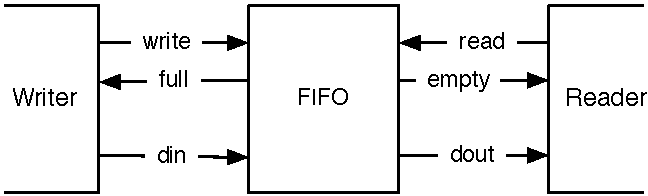
\includegraphics[scale=\scale]{../figures/fifo}
  \caption{A writer, a FIFO buffer, and a reader.}
  \label{fig:fifo}
\end{figure}
\begin{itemize}
\item FIFO style queues between a sender and a receiver
\item The sender/writer enqueues/writes into the Queue
\item The receiver/reader dequeues/reads from the Queue
\item Can \emph{even out} bursty traffic
\end{itemize}
\end{frame}

\begin{frame}[fragile]{Queues}
\begin{itemize}
\item Used when there is bursty traffic
\begin{itemize}
\item E.g., on a serial port
\item Write faster from CPU than serial can send
\item Receive data when CPU is busy with other stuff
\end{itemize}
\item But can fill up when the sender is continuously \emph{faster}
\item Showing implementation variations in the Chisel book
\begin{itemize}
\item Bubble FIFO (was proposed in lab 5)
\item double buffer, memory-based, ...
\end{itemize}
\end{itemize}
\end{frame}

\begin{frame}[fragile]{Bubble FIFO Example}
\begin{itemize}
\item FIFO interface
\shortlist{../code/fifo_io.txt}
\item Abstract base class (with some common code)
\shortlist{../code/fifo_abstract.txt}
\item \href{https://github.com/schoeberl/chisel-book/blob/master/src/main/scala/fifo/fifo.scala}{FIFO code}
\end{itemize}
\end{frame}

\begin{frame}[fragile]{Bubble FIFO}
\begin{itemize}
\item Simple, easy to understand
\item Uses minimal resources
\item However, each buffer stage has to toggle between empty and full
\item Maximum bandwidth is one word every two clock cycles
\item When full, needs N cycles for a restart
\begin{itemize}
\item The free element \emph{bubbles} towards the input
\end{itemize}
\item Better solutions
\begin{itemize}
\item Double buffer
\item Memory with read and write pointers
\end{itemize}
\end{itemize}
\end{frame}

\begin{frame}[fragile]{Use Inheritance}
\begin{itemize}
\item Defined an abstract base class for the FIFO and extend it
\begin{itemize}
\item Also use traits to inherit from several sources
\end{itemize}
\item Learn from software development to share code
\item We select the implementation by the type
\begin{chisel}
class DoubleBufferFifo[T <: Data](gen: T, depth: Int) extends Fifo(gen: T, depth: Int) {
...
class RegFifo[T <: Data](gen: T, depth: Int) extends Fifo(gen: T, depth: Int) {
...
class MemFifo[T <: Data](gen: T, depth: Int) extends Fifo(gen: T, depth: Int) {
...
\end{chisel}
\item Explore the different implementation details in Section 11.3 of the Chisel book

\end{itemize}
\end{frame}

\begin{frame}[fragile]{Chisel \code{Queue}}
\begin{itemize}
\item Chisel has a \code{Queue}
\item Interfaces are \code{DecoupledIO}s
\item Specify type and number of entries Queue(UInt(4.W), 8)
\item Optional arguments
\begin{itemize}
\item \code{pipe}: if full, allow concurrent enqueue and dequeue
\item \code{flow}: if empty, enqueued value available immediately for dequeue
\end{itemize}
\item What is the implementation? Resources? Throughput?
\end{itemize}
\begin{chisel}
val q = Module(new Queue(UInt(), 16))
q.io.enq <> producer.io.out
consumer.io.in <> q.io.deq
\end{chisel}
\end{frame}

\begin{frame}[fragile]{Connect a Network-on-Chip}
\begin{itemize}
\item n x n router in bi-thorus configuration
\item Each raouter has 4 + 1 ports: North, South, West, East, and local
\item Use a helper function \code{connect(...)}
\end{itemize}
\begin{chisel}
  def connect(r1: Int, p1: Int, r2: Int, p2: Int): Unit = {
    net(r1).io.ports(p1).in := net(r2).io.ports(p2).out
    net(r2).io.ports(p2).in := net(r1).io.ports(p1).out
  }

  for (i <- 0 until n) {
    for (j <- 0 until n) {
      val r = i * n + j
      connect(r, EAST, i * n + (j + 1) % n, WEST)
      connect(r, SOUTH, (i + 1) % n * n + j, NORTH)
    }
  }
\end{chisel}
\end{frame}

\begin{frame}[fragile]{Why Open Source?}
\begin{itemize}
\item Can improve your visibility
\item Add your GitHub repos to your CV
\item When hiring, I look up GitHub contributions
\item You can get help from the community
\item I got free translations of my Chisel book
\item Why not?
\begin{itemize}
\item You already use open-source tools and libraries
\item So return some to the community
\item Even in a company, if there is no patent
\item Oticon contributes to Zephyr
\end{itemize}
\end{itemize}
\end{frame}


\begin{frame}[fragile]{Open-Source Licensing}
\begin{itemize}
\item You own the copyright when creating code
\begin{itemize}
\item Hardware is different in DK, so it is blurry
\item Maybe your employer owns the copyright (not at DTU)
\end{itemize}
\item A license grants others to use and change your code
\begin{itemize}
\item Different licenses have different permissions and restrictions
\end{itemize}
\item When releasing, add a license to your repo
\begin{itemize}
\item Have it clearly visible (e.g., as LICENSE in the project root)
\item GitHub will detect it
\end{itemize}
\end{itemize}
\end{frame}


\begin{frame}[fragile]{License Types}
\begin{itemize}
\item BSD and MIT
\begin{itemize}
\item Commonly used, good for academic
\item Basically, use my stuff, but don't sue me
\item Can also be used in a commercial product (e.g., network stack)
\end{itemize}
\item GPL
\begin{itemize}
\item Commonly used in software
\item Copyleft means you have to make all changes available
\item Some companies have restrictions on using GPL software
\end{itemize}
\item Apache
\begin{itemize}
\item Similar to BDS and MIT
\item Includes explicit patent protection
\end{itemize}
\end{itemize}
\end{frame}


\begin{frame}[fragile]{Documentation}
\begin{itemize}
\item Summarize the purpose of your project
\item Instruct how to use it
\item List dependencies
\item Good documentation:
\begin{itemize}
\item May attract users
\item May even attract contributors
\item Forces you to rethink your project
\end{itemize}
\item Start early with the documentation
\end{itemize}
\end{frame}


\begin{frame}[fragile]{README.md}
\begin{itemize}
\item Well-suited for small to medium projects
\item Immediately visible on GitHub
\item Use Markdown for simple formatting
\item Include figures, best in SVG
\item I will consider the README as part of the grade
\begin{itemize}
\item Don't wait till the final week!
\end{itemize}
\end{itemize}
\end{frame}

\begin{frame}[fragile]{On the Project}
\begin{itemize}
\item Next week is your initial presentation
\item No lab
\end{itemize}
\end{frame}

\begin{frame}[fragile]{The Exam and Grading}
\begin{itemize}
\item Grade is based on:
\begin{itemize}
\item The project (source code)
\item The documentation
\item The presentations
\end{itemize}
\item Final week: your project presentation (= exam)
\item No report to be written
\item But I expect a very detailed README.md
\begin{itemize}
\item Explain what it does and how to use it
\item State your usage of AI/LLM
\end{itemize}
\end{itemize}
\end{frame}

\begin{frame}[fragile]{Summary}
\begin{itemize}
\item We use Scala to write hardware generators
\item Get started with your project
\item Collect ideas for more productive generator code
\item Did you find some Scala tricks that I did not present?
\begin{itemize}
\item Add to our shared Google Docs
\item Also, what you are missing
\end{itemize}
\item Use ready/valid interfaces (DecoupledIO)
\item Use queues, arbitration
\item Go open source!
\item Next week: guest lecture by Ioannis on LLM usage at Microhip
\end{itemize}
\end{frame}

\end{document}

\begin{frame}[fragile]{Title}
\begin{itemize}
\item abc
\end{itemize}
\end{frame}
